\documentclass[crop,tikz]{standalone}% 'crop' is the default for v1.0, before it was 'preview'
\usepackage{tikz,calc,pgfplots}
\usetikzlibrary{calc}
\begin{document}

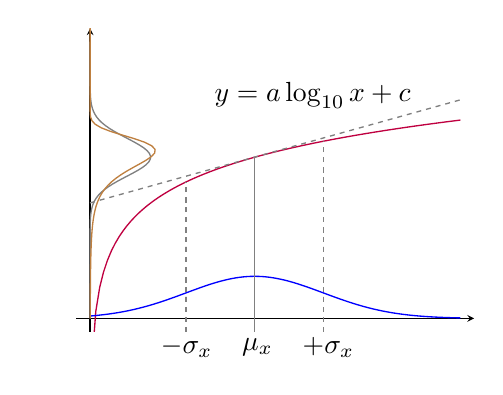
\begin{tikzpicture}[scale=0.6,
declare function={ 
	mu = 6;
	sig = 2.5;
	G(\x) = 4*log10(\x)+3;		
	X(\x) = 1/(sig*sqrt(2*pi))*exp(-((\x-mu)^2)/(2*sig^2)); 				
	hinvd(\y) = (2^((\y-11)/4)) * (5^((\y-3)/4)) * ln(10);
	hinv(\y) = 10^((\y-3)/4);
	Y(\y) = abs(hinvd(\y))*(1/(sig*sqrt(2*pi))*exp(-((hinv(\y)-mu)^2)/(2*sig^2)));
	J = 4/(mu*ln(10)); % Jacobian of prop function evaluated at mean value
	linG(\x) = J*\x+4.38;		
	sigProp = sig*J; % propagated standard dev
	muProp = 4*log10(mu)+3; % propagated mean				
	Yy(\y) = 1/(sigProp*sqrt(2*pi))*exp(-((\y-muProp)^2)/(2*sigProp^2));
}
]

\begin{axis}[thick,
width=10cm,
height=8cm,
samples = 100,
%                     xlabel = $x$,
%                     ylabel = $y$,
xmin = -0.5,
xmax = 14,
ymin = -0.5,
ymax = 11,
axis x line = middle,
axis y line = middle,
ticks = none]

\addplot[purple,domain=-0.5:13.5] plot (\x, {G(\x)} );
\addplot[gray,dashed,domain=-0:13.5] plot (\x, {linG(\x)} );
\addplot[blue,variable=\x,domain=-0:13.5] plot( {\x} , {10*X(\x)} ); 
\addplot[gray,variable=\y,domain=-0:10.5] plot( {4*Yy(\y)} , {\y} );             	                     	          
\addplot[brown,variable=\y,domain=-0:13.5] plot( {4*Y(\y)} , {\y} );           


\addplot[gray,dashed,variable=\y,domain=-0.5:{G(mu+sig)}] plot ({mu+sig}, {\y});
\addplot[gray,variable=\y,domain=-0.5:{G(mu)}] plot ({mu}, {\y});
\addplot[gray,dashed,variable=\y,domain=-0.5:{G(mu-sig)}] plot ({mu-sig},{\y});  	            	          
%   	          \addplot[gray,dashed,variable=\x,domain=-0.5:{(mu+sig)}] plot ({\x}, {G(mu+sig)});
%   	          \addplot[gray,variable=\x,domain=-0.5:{(mu)}] plot ({\x}, {G(mu)});
%   	          \addplot[gray,dashed,variable=\x,domain=-0.5:{(mu-sig)}] plot ({\x}, {G(mu-sig)});  	   
\end{axis}

\node at (5.3334,-0.3332) {$+\sigma_x$};
\node at (2.3334,-0.3332) {$-\sigma_x$};
\node at (3.8334,-0.3332) {$\mu_x$};
% \node at (5.5,5) {$y=Mx+c$};
\node at (5,5) {$y=a \log_{10}x+c$};
 \node at (-0.2,3.55) {$\color{white}\mu_y$};
 \node at (-0.3,3.95) {$\color{white}+\sigma_y$};
 \node at (-0.3,3.15) {$\color{white}-\sigma_y$};
\end{tikzpicture}
\end{document}